

\documentclass[a4paper]{report}
\usepackage[margin=1in]{geometry}
\usepackage{polyglossia}
\usepackage{csquotes}
\setdefaultlanguage[variant=british]{english}
\usepackage{titlepic}
\usepackage{graphicx}
\usepackage{xcolor}
\usepackage{amsfonts, amsmath, amssymb}
\usepackage{float} %ensures that figures / tables can be floated on page
\usepackage{fancyref}
\usepackage[sorting=none,backend=biber]{biblatex}
\usepackage{notoccite}
\addbibresource{references.bib}

%%% run    biber e4dse_jba.bcf     to update references

\newcommand{\MATLAB}{\textsc{Matlab}}
\newcommand{\sbul}{\begin{itemize}}
\newcommand{\ebul}{\end{itemize}}

\usepackage{setspace}
\onehalfspacing % line spacing (is equal to baselinestretch 1.33)

\usepackage[numbered,framed]{matlab-prettifier}
\lstset{
  language           = Matlab,
  style              = Matlab-editor,
  basicstyle         = \mlttfamily,
  escapechar         = `,
  mlshowsectionrules = true
}

%\lstloadlanguages{[ISO]C++,[99]C}



\usepackage{listings}

\definecolor{commentgreen}{RGB}{2,112,10}
\definecolor{eminence}{RGB}{108,48,130}
\definecolor{weborange}{RGB}{255,165,0}
\definecolor{frenchplum}{RGB}{129,20,83}
\definecolor{backgroundColour}{rgb}{0.95,0.95,0.92}

\lstdefinestyle{C++}{
    language=C++,
    escapechar=\%,
    backgroundcolor=\color{backgroundColour},
    commentstyle=\color{commentgreen},
    keywordstyle=\color{eminence},
    stringstyle=\color{red},
    basicstyle=\small\ttfamily,
    emph={int,char,double,float,unsigned,void,bool,uint32_t,uint16_t},
    emphstyle={\color{blue}},
    breakatwhitespace=false,
    breaklines=true,
    captionpos=b,
    keepspaces=true,
    numbers=left,
    numbersep=5pt,
    showspaces=false,
    showstringspaces=false,
    showtabs=false,
    tabsize=2,
    showstringspaces=false
}

\usepackage[binary-units=true]{siunitx}
\sisetup{detect-all}

%\definecolor{vertmatlab}{RGB}{28,160,55}
%\definecolor{mauvematlab}{RGB}{155,71,239}
%\definecolor{fond}{RGB}{246,246,246}
\definecolor{lightgray}{gray}{0.7}

\sloppy
%\setlength{\parindent}{0pt}

\usepackage{titlesec}
\titleformat{\chapter}{\huge\bf}{\thechapter.}{20pt}{\huge\bf}
\titleclass{\chapter}{straight}

\usepackage[colorlinks,citecolor=blue,linkcolor=black,urlcolor=blue]{hyperref}


\usepackage{glossaries}
%\usepackage[toc]{glossaries}
\makeglossaries
\loadglsentries{glossary}

%%%% run makeglossaries e4dse_jba.glo if any changes to glossary file.

%% Own operators
\DeclareMathOperator{\Rot}{Rot}
\newcommand{\matr}[1]{\mathbf{#1}}
%%


%%%%%%
\author{Janus Bo Andersen\thanks{Student number: JA67494. AU-number: AU191419. E-mail: ja67494@post.au.dk}}
\titlepic{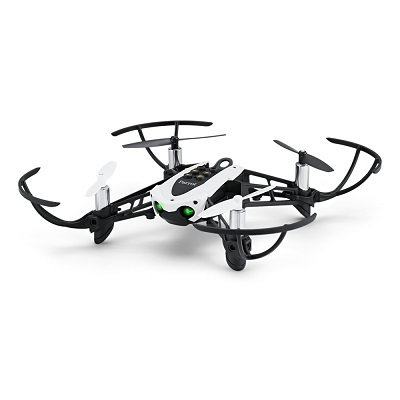
\includegraphics[width=\textwidth]{img/mambo.jpg}}


%%%%%%
\begin{document}

\pagenumbering{roman}
\title{Quadrotor control: Control project in E4DSE}
\maketitle

\tableofcontents

\newpage
\printglossaries

\newpage
\pagenumbering{arabic}


\chapter{Introduction to the project}

This project is part of the course E4DSE (Dynamic Systems) at Aarhus University, Campus Herning.
Scope and focus of the project was chosen by the author with the purpose to demonstrate basic control theory in the context of a physical system.
The covid-19 close-down meant that the otherwise mandatory lab part was omitted, allowing a more optional approach to the project.

The aim of this project is to develop and test parts of a flight controller for a quadrotor drone.
Models for the flight dynamics of a quadrotor, and the controllers to achieve control aims, are discussed and implemented in Simulink and \MATLAB.
%Controllers for different parts of the flight dynamics are implemented and tested.
%Finally, a physical drone, the Parrot Mini Mambo (as seen on the cover page), is used to test the performance of the implemented controllers on a real physical system.

The project report was written in English so established terminology can be leveraged more freely in the report. 
Especially within flight dynamics and parts of control theory, terminology relies heavily on English.
Also, the course co-responsible is a non-Dane.
Further, the author intends to continue work on this project and potentially use it beyond E4DSE.
All figures and code was developed by the author.

%The tex-files for the report, draw.io-files for all figures, \MATLAB~code and Simulink models are available on github at \url{https://github.com/janusboandersen}.

\section{Introduction to quadrotors}

A quadrotor is a type of drone that achieves lift and propulsion by driving four independent rotors. 
These are mounted on opposing sides of a rigid airframe.
A single rotor only turns in one direction, but the rotors have pairwise reversed directions of rotation to balance total torque on the body.
Unlike a helicopter, the rotor blades of a quadrotor cannot be pitched, and thrust is therefore controlled fully by the angular velocity of the rotors.

Flight is controlled by translation in the $x,y,z$ directions and through rotations of the airframe (yaw, roll, pitch). 
As the quadrotor only has 4 rotors (actuators) to to navigate in the 6 \gls{DoF} of the physical environment, it is under-actuated.

In many modern applications, the quadrotor is a \gls{UAV} and is possibly also flying autonomously.
For the above and many other reasons, feedback control is essential in flying and navigating the drone.


\section{Problem statement and delimitations}

The idea of this project is to balance the focus between \textit{developing} the dynamical models of a quadrotor and \textit{applying} control theory to the dynamic system. For this reason, the dynamical models are developed in one and two dimensions, in order to have sufficient ``room'' to also give focus to application of control theory.
The geometry and linear algebra needed as background is developed in more general terms, so the third dimension could be added later.

\textbf{Project aim:}
The physical, dynamical model of a quadrotor are to be described in one and two dimensions. Using these models, controllers are to be developed and implemented to achieve control objectives.

\textbf{Control objectives are:}
\sbul
\item Navigate to and maintain hover flight at given vertical position.
\item Navigate to and maintain hover flight at given vertical and horizontal position.
%\item Navigate to and maintain hover flight at given position in 3-dimensional space.
\item Achieve the above objectives with performance that is comparable to a real quadrotor, i.e. rise times, settling times, etc.
\ebul

\textbf{Delimitations:}
The control focus is to obtain control inputs to manoeuvre the quadrotor drone.
Sensor inputs are taken as given, assuming that these are ideal and thus providing unity feedback, i.e. the sensors have transfer functions of unity.
%In the physical implementation, sensor readings are obtained through the manufacturer's code. The Kalman filtering required to obtain good estimates based on data from the \gls{IMU}, the downward-facing camera and the air pressure sensor, is a complex topic that could be the focus of another full report.

In 1-dimensional space with a \gls{SISO} model, control can be done using ``classical control'' methods. 
This is also the case in 2 dimensions, if the equations of motion are linearized and decoupled. 

When equations are coupled, and potentially also in 3 dimensions, and maybe with more complex control goals, it becomes more natural to use the state-space representation for the \gls{MIMO} models. This is not a part of the E4DSE curriculum. 
Nonetheless, parts of this approach have been employed as possible where necessary.

The author has relied on results from linear algebra, equivalent in scope to the course ETALA. It is not the purpose to review linear algebra, and little focus is given to explaining these concepts.


\chapter{Overview of geometry, linear algebra and physics to model a quadrotor}

\section{Reference frames and translations}
Two right-handed frames of reference are used to model quadrotor dynamics; 
The world frame, $\mathcal{A}$, is an \textit{inertial frame}, and the body frame, $\mathcal{B}$, is attached to the quadrotor, with origin in the center of mass, similar to \cite[p. 310]{Powers2015}.
Each frame is chosen as an orthogonal basis in $\mathbb{R}^3$. $\mathcal{A}$ is the standard basis.

\begin{figure}[H]
\centering
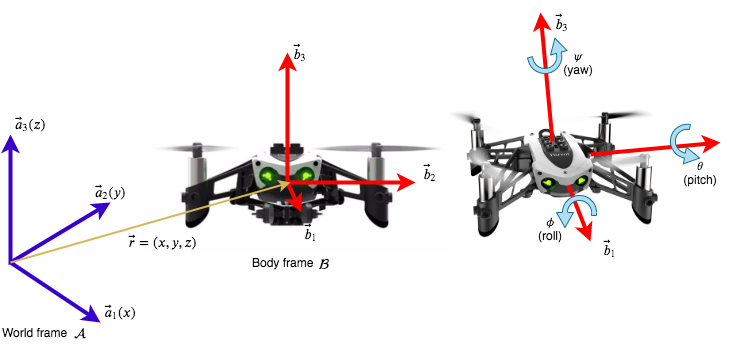
\includegraphics[width=14cm]{img/frames.png}
\caption{Frames of reference\label{fig:frames}}
\end{figure}

The body frame translates and rotates with the center of mass of the quadrotor. 
The position vector $\vec{r}=(x, y,z)$ measures the displacement of the rigid body \textit{relative} to frame $\mathcal{A}$. 

\section{Rotations and rotation matrices}
There are a few ways to describe rotations of a rigid body.
The purpose is to convert the coordinates of a vector in one frame to coordinates in the other frame. 
The most intuitive is by \textbf{Euler angles}, using a sequence of three rotations about three non-collinear axes, with which any rigid body rotation can be modelled\footnote{
Except for certain configurations that result in a degenerate system if two axes become collinear.
This is similar to the ``Gimbal lock'' phenomenon. 
Also similar to how the the latitude-longitude coordinate system degenerates at the geographic poles.
Here, longitude is no longer unique, and no reverse transformation can give unique coordinates.
}.
Rotations in general are not commutative.
A rotation can be composed in any order. In this project, the Euler angles are applied in the order $Z$-$X$-$Y$: 
Yaw (by angle $\psi$ around $\vec{b}_3$),
roll (by angle $\phi$ around $\vec{b}_1$) and
pitch (by angle $\theta$ around $\vec{b}_2$) \cite[p. 313]{Powers2015}.

For example, a roll by $\phi$ around the $x$-axis is $\Rot(x, \phi)$. This can be represented by a rotation matrix, which describes the coordinates of the new rotated basis in terms of the world frame. An example process to get from $\mathcal{A}$ to $\mathcal{B}$ when rotating by $\phi$ is shown in the figure below.

\begin{figure}[H]
\centering
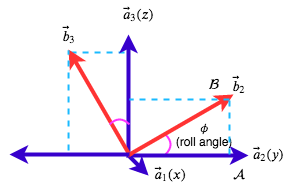
\includegraphics[width=7cm]{img/rotations.png}
\caption{Rotation by $\phi$ around the $x$-axis.\label{fig:rotations}}
\end{figure}

The coordinates of the basis of the $\mathcal{B}$-frame before the rotation is the same as the standard basis

\begin{equation}
\vec{a}_1 = 
\begin{bmatrix}
1 \\
0 \\
0
\end{bmatrix} 
, \vec{a}_2 =  
\begin{bmatrix}
0 \\
1 \\
0
\end{bmatrix}
, \vec{a}_3 = 
\begin{bmatrix}
0 \\
0 \\
1
\end{bmatrix}
\end{equation}

After the rotation, the new basis is found by simple trigonometry 

\begin{equation}
\vec{b}_1 = 
\begin{bmatrix}
1 \\
0 \\
0
\end{bmatrix} 
, \vec{b}_2 =  
\begin{bmatrix}
0 \\
\cos \phi \\
\sin \phi
\end{bmatrix}
, \vec{b}_3 = 
\begin{bmatrix}
0 \\
-\sin \phi \\
\cos \phi
\end{bmatrix}
\end{equation}

So this rotation is described by the rotation matrix

\begin{equation} \label{eq:rotx}
\Rot(x, \phi) = \matr{R}=
\begin{bmatrix}
1 & 0 & 0 \\
0 & \cos \phi  & -\sin \phi\\
0 & \sin \phi & \cos \phi
\end{bmatrix} 
\end{equation}

A point $\vec{p} \in \mathbb{R}^3$ can be described \textsl{in terms of} $\mathcal{B}$. Then it has a unique coordinate vector $[\vec{p}]_\mathcal{B}=[c_1, c_2, c_3]^T \in \mathbb{R}^3$ \cite[p. 218]{lay}.
To get the coordinates of this point in the standard basis, i.e. with respect to $\mathcal{A}$, the change-of-basis matrix is the rotation matrix $\matr{R}$. So we return to the standard basis by taking a linear combination of the columns of the rotation matrix \cite[p. 243]{lay}, that is:

\begin{equation}
\vec{p} = [\vec{p}]_\mathcal{A} = \matr{R} [\vec{p}]_\mathcal{B}
\end{equation}

The axes \textit{of this rotation matrix} are not collinear, so the inverse exists. Because rotation matrices are orthogonal, it is true that $\matr{R}^{-1} \matr{R} = \matr{R}^{T} \matr{R} = \matr{I}$. Given a point $\vec{p}$, the coordinate vector in $\mathcal{B}$ can be found as 

\begin{equation}
[\vec{p}]_\mathcal{B} = \matr{R}^T \vec{p}
\end{equation}

An example is a rotation by $\phi=45$°, then $\cos \phi = \sin \phi = 1/\sqrt{2}$.
Take a point in terms of the rotated basis, say $[\vec{p}]_\mathcal{B} = [0, 1/\sqrt{2}, 1/\sqrt{2}]^T$, i.e. a unit vector in the $yz$-plane at a 45° angle to $\vec{b}_2$.
Then $\vec{p}=\matr{R} [\vec{p}]_\mathcal{B} = [0, 0, 1 ]^T$. This is $1 \cdot \vec{a}_3$, as would be expected.
Also, $\matr{R}^T \vec{a}_3 = [0, 1/\sqrt{2}, 1/\sqrt{2}]^T$.

\section{ZXY rotations}

As mentioned, the order of application of the Euler angles is Z-X-Y.
So rotation matrices are needed to model these three rotations. Rotation matrices for $\Rot(y, \theta)$ and $\Rot(z, \psi)$ are found in a similar way to $\Rot(x, \phi)$ from the previous section. The three matrices are shown below:

\begin{equation}
\Rot(x, \phi)=
\begin{bmatrix}
1 & 0 & 0\\
0 & \cos\phi & -\sin\phi \\
0 & \sin\phi & cos\phi
\end{bmatrix},
\Rot(y, \theta)=
\begin{bmatrix}
\cos\theta & 0 &  \sin\theta \\
0 & 1 & 0 \\
-\sin\theta & 0 & \cos\theta
\end{bmatrix},
\Rot(z, \psi)=
\begin{bmatrix}
\cos\psi & -\sin\psi &  0\\
\sin\psi & \cos\psi & 0 \\
0 & 0 & 1
\end{bmatrix}
\end{equation}

In a pure rotation, one point remains fixed (origin). 
A rigid rotation is a linear transformation of a rigid body so the body does not deform, i.e. distances between points (norms) and angles between points (cross-products) are preserved in the rigid body\footnote{
Rotation matrices belong to the 3D rotation group, $SO(3)$. They are orthogonal matrices with the following characteristics: 
$\det{\matr{R}}=1$ i.e. no volumetric change due to the transformation and $R(\vec{p}\times\vec{q})=R(\vec{p}) \times R(\vec{q})$ and due to orthogonality $\matr{R}^T \matr{R} = \matr{R}^{-1} \matr{R} = \matr{I}$. The inverse of a rotation matrix is also a rotation matrix, and ``undoes'' the rotation of $\matr{R}$.
}. 

Transformations are composed right-to-left, and ``undone'' in the reverse order.
So to return to the standard basis from a ZXY-rotated frame, the following composite matrix transforms a coordinate vector in
$\mathcal{B}$-coordinates to $\mathcal{A}$-coordinates:

\begin{equation}
\matr{R}=\Rot(z, \psi)  \Rot(x, \phi) \Rot(y, \theta)
\end{equation}

Using \MATLAB, the composed transformation can be seen (similar result as given by \cite[p. 313]{Powers2015});
\begin{lstlisting}[language=Matlab, style=Matlab-editor]
 % roll (about b1 or x), pitch (about b2 or y), yaw (about b3 or z)
f = sym('phi');  t = sym('theta'); p = sym('psi'); 
R_x = [1 0       0; 
       0 cos(f) -sin(f);
       0 sin(f)  cos(f)];
R_y = [cos(t) 0  sin(t); 
       0      1  0; 
      -sin(t) 0  cos(t)];
R_z = [cos(p) -sin(p) 0; 
       sin(p)  cos(p) 0;
       0       0      1];
R = R_z * R_x * R_y
\end{lstlisting}

\begin{equation}
\left(\begin{array}{ccc}
\mathrm{cos}\left(\psi \right)\,\mathrm{cos}\left(\theta \right)-\mathrm{sin}\left(\phi \right)\,\mathrm{sin}\left(\psi \right)\,\mathrm{sin}\left(\theta \right) & -\mathrm{cos}\left(\phi \right)\,\mathrm{sin}\left(\psi \right) & \mathrm{cos}\left(\psi \right)\,\mathrm{sin}\left(\theta \right)+\mathrm{cos}\left(\theta \right)\,\mathrm{sin}\left(\phi \right)\,\mathrm{sin}\left(\psi \right)\\
\mathrm{cos}\left(\theta \right)\,\mathrm{sin}\left(\psi \right)+\mathrm{cos}\left(\psi \right)\,\mathrm{sin}\left(\phi \right)\,\mathrm{sin}\left(\theta \right) & \mathrm{cos}\left(\phi \right)\,\mathrm{cos}\left(\psi \right) & \mathrm{sin}\left(\psi \right)\,\mathrm{sin}\left(\theta \right)-\mathrm{cos}\left(\psi \right)\,\mathrm{cos}\left(\theta \right)\,\mathrm{sin}\left(\phi \right)\\
-\mathrm{cos}\left(\phi \right)\,\mathrm{sin}\left(\theta \right) & \mathrm{sin}\left(\phi \right) & \mathrm{cos}\left(\phi \right)\,\mathrm{cos}\left(\theta \right)
\end{array}\right)
\end{equation}

Such matrices can be used to convert force vectors in one fram to another. Conversely, if this matrix is known from sensor data, the Euler angles can be backed out. Here, starting in row 3, column 2 to get $\phi$. Notice, for this composed rotation there are 9 entries in a $3 \times 3$ matrix, but only 3 Euler-angles, so the rotation matrix has redundant information.

\section{Translational and rotational kinematics}

Time derivatives are denoted with dots, e.g. $\ddot{\vec{r}}=\frac{d^2}{dt^2}\vec{r}=\vec{a}$. 
For translational motion, the kinematics of the rigid body quadrotor in the inertial frame $\mathcal{A}$ are governed by Newton's 2nd Law:

\begin{equation}\label{eq:N2}
\sum \vec{F} = m \ddot{\vec{r}}
\end{equation}

The rotational kinematics around center of mass of the drone, along principal axes ($x$, $y$, $z$), are 
\begin{equation}\label{eq:rot_kinematics}
\sum \vec{\tau} = \matr{I_C} \vec{\alpha}
\end{equation}

Meaning that the resultant (vectorial) sum of torques drives angular acceleration, $\vec{\alpha}=\dot{\vec{\omega}}$, along the principal axes, in relation to the inertia of the rigid body. $\matr{I_C}$ is the inertia tensor along principal axes:

\begin{equation}
\matr{I_C} = 
\begin{bmatrix}
I_{xx} & 0 & 0\\
0 & I_{yy} & \\
0 & 0 & I_{zz}
\end{bmatrix}
\end{equation}

A few further topics needed for 3D kinematics have been omitted. One key ``ingredient'' needed for 3D is the rate of change of rotations and conversions between the Euler rates used in the models and angular body rates, i.e. acting instantaneously on the body and measured by e.g. the \gls{IMU}.

\section{Physical properties of the quadrotor}

A Parrot Mini Mambo drone is modelled in this project. It is the type shown on the cover page and in various figures. The author has acquired such a drone, and experimented with some of the flight controllers on it. So it makes sense to use the physical characteristics of this. The physical properties have been extracted from \cite{quadcopterproject} and are shown below:

\begin{table}[h!]
\centering
\begin{tabular}{ |p{7cm}||p{3cm}|p{3cm}|  }
\hline
\multicolumn{3}{|c|}{Parrot Mambo Mini} \\
\hline
Property & Value & SI unit \\
\hline
Mass, $m$                               & \num{63.0e-3}    & \si{\kilo\gram} \\
Inertia about x-axis, $I_{xx}$  & \num{5.83e-05} & \si{\kilo\gram\meter\squared} \\
Inertia about y-axis, $I_{yy}$  & \num{7.17e-05} & \si{\kilo\gram\meter\squared} \\
Inertia about z-axis, $I_{zz}$  & \num{1.00e-04} & \si{\kilo\gram\meter\squared} \\
Distance from center of mass to rotor, $L$  & \num{6.00e-2} & \si{\meter}  \\
\hline
\end{tabular}
\caption{Physical properties of the modelled quadrotor \label{fig:physical_props}}
\end{table}

\chapter{Quadrotor in one dimension}

A first interesting case is to model the quadrotor purely in the $z$-direction.
Here, the drone can lift off and maintain a hover at a given vertical position.

\section{Dynamics}

The free-body diagram below shows the quadrotor in a hover configuration at $z=$ \SI{0}{\meter}. 
The thrusts from the rotors are equal and add up to a combined force $\vec{F}$ acting on the center of mass.
The mass of the drone is stated in table \ref{fig:physical_props}.
When $\vec{F}=m g \vec{a}_3$, the drone maintains a hover.

\begin{figure}[H]
\centering
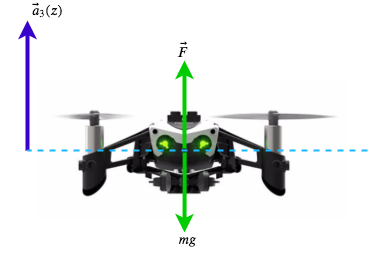
\includegraphics[width=8cm]{img/phy_1d.png}
\caption{Free-body of quadrotor in 1 dimension\label{fig:phy_1d}}
\end{figure}

A simple model is to assume small deviations from this hover configuration. So a control input is chosen as $u(t)=F(t)-mg$. 
This is a variable substitution in order to get a linear system\footnote{
The system is nonlinear due to the constant term $mg$.
A linear system $f$ with inputs $u$ and $v$ must obey additivity $f(u+v)=f(u)+f(v)$ and homogeneity $f(\alpha u) = \alpha f(u)$.
}. 
A positive control input is application of force such that the drone will increase its vertical position.

At hover, $u(0)=0$, and so are the initial conditions of position, velocity and acceleration:
$z(0)=0$, $\dot{z}(0)=0$ and  $\ddot{z}(0)=0$.

It is assumed that drag is negligible as the drone moves vertically in the air; otherwise add damping by including the force $F_f = b \dot{z}$ in the direction opposite to travel.
The linear 2nd order \gls{ODE} of this physical system using eq. \ref{eq:N2} is

\begin{equation} \label{eq:model_1d}
\sum \vec{F} = u(t) = m \ddot{z}
\end{equation}

\section{Transfer function and s-domain model}

The simple linear model transformed using Laplace is 

\begin{equation} \label{eq:model_1d_s}
m s^2 Z(s) = U(s)
\end{equation}

The transfer function of the plant is given below. The plant is the relation of the vertical position (output) of the quadrotor as excess force is applied (input).

\begin{equation} \label{eq:model_1d_tf}
G(s) = \frac{Z(s)}{U(s)} = \frac{1}{m} \frac{1}{s^2}
\end{equation}

Notice the double integrator in the plant. This of course corresponds to the double integration required to solve equation \ref{eq:model_1d}. The system is \gls{BIBO} \textbf{unstable} as there is no damping in the system. Physcially, the intuition is that any bounded input of net force, say $u(t)>0$ briefly, will impart a brief acceleration on the body. Therefore the quadrotor will continue to move at a constant velocity indefinitely, due to Newton's 1st law, and the output (position) will increase unbounded.

As the goal is to achieve a hover at time $t=t^*$ at position $z(t^*)=z_\text{ref}$, it must also be ensured that $\dot{z}(t^*)=0$ so the quadrotor is not moving. \\ \\

\textbf{Stability margins:}
With a double integrator plant, i.e. two poles at the origin, the phase of the open-loop system is \SI{-180}{\degree}. The phase-margin is $\text{PM}=0$.
A positive margin, $\text{PM}>0$, is required for stability \cite[p. 349]{franklin}.
$\text{PM}$ is measured where $|G(s)|=1$, as $\text{PM} = \angle G(s) + 180°$. But at any point $\angle G(s) = -180°$, because phase is constant \SI{-180}{\degree} for this plant.

If the loop is closed, the characteristic equation becomes $1+G(s)=0$, and
when $\angle G(s) = -180°$ and $|G(s)|=1$, the characteristic equation is $1+\angle G(s)|G(s)| = 1-1 = 0$.
The significance of this is: As there is $0$ phase margin, there is zero margin before the system becomes unstable. 
No value of gain can change that.
So to obtain a stable system, zero(s) must be added (e.g. derivative gain).


\section{Controller design}

The controller must convert position errors into control actions. It must do so with performance that matches the design goals.

\subsection{A P-controller gives oscillatory system}
With a P-controller, the output would be undamped and oscillatory: The quadrotor would ``overshoot'' and ``undershoot'' indefinitely, as the velocity of the drone upon reaching the set-point would be \textit{non-zero}.  Physically, it would be like an ideal spring attached to the quadrotor.

This can be seen from a root locus analysis, let proportional gain $K_p$ be the parameter varied. 
The closed-loop system with a P-controller is

\begin{equation}
G_{cl}(s) = \frac{Y(s)}{R(s)} = \frac{K_p G(s)}{1 + K_p G(s)}
\end{equation}

The closed loop system poles are the roots of $1+K_p G(s) = 0$. In root locus form

\begin{equation}
1 + K_p L(s) = 0 \longrightarrow ms^2 + K_p = 0
\end{equation}

The roots are $r = \pm \frac{\sqrt{-4mK_p}}{2m}$. 
So for any positive value of $K_p$, the roots will be purely imaginary. 
For any positive value of $K_p$, this is an oscillatory system without damping (real part of poles is zero).
This we already knew from the stability margins above.


\subsection{A PD-controller dampens the double-integrator system}

To damp the motion, i.e. get $\dot{z}(t^*)=0$ at some time $t^*$ when the quadrotor is at a hover, a PD-controller must be used. 
I.e. we add a zero to the open loop gain.
Physically, this is like adding damping, which will result in dissipation of energy.

The desired hover position is $z_\text{ref}$ and the current position is $z(t)$. The position error of the quadrotor is $e(t)=z_\text{ref} - z(t)$.
The PD-controller $h$ works on the error with proportional and derivative gain as

\begin{equation} \label{eq:PD_1d_verbose}
h(t) = K_p e(t) + K_d \dot{e}(t) = K_p ( z_\text{ref} - z(t) ) + K_d \frac{d}{dt}( z_\text{ref} - z(t) )
\end{equation}

So this is clearly a 1st order \gls{ODE}. Assuming that the set-point $z_\text{ref}$ is constant, the time derivative of the error is $\dot{e}(t) = -\dot{z}(t)$. So derivative gain will reduce the control input at high velocities, resulting in a dampening of the velocity and position of the quadrotor.
The output of the PD-controller is

\begin{equation} \label{eq:PD_1d_simple}
h(t) = K_p e(t) - K_d \dot{z}(t)
\end{equation}

This \gls{ODE} in $z$ or in $e$ can be solved to get the controller. In the s-domain, the controller has the following transfer function by way of transformation of eq. \ref{eq:PD_1d_verbose}, see e.g. \cite[p. 201]{franklin}

\begin{equation} \label{eq:PD_1d_s}
PD(s) = \frac{H(s)}{E(s)} = K_p + K_d s
\end{equation}

\subsection{Stability}

With a PD-controller, the characteristic equation is $1+ PD(s)\cdot G(s) = 0$.
In polynomial form, the characteristic equation is $ms^2 + K_d s + K_p = 0$.
The roots of this equation are

\begin{equation} \label{eq:cl_poles}
r_{1,2} = -\frac{K_d}{2m} \pm \frac{\sqrt{K_d^2 - 4 m K_p}}{2m}
\end{equation}

The roots of the characteristic equation are the system poles.
So $K_p$ and $K_d$ must be chosen so the poles $s=r_1$ and $s=r_2$ lie in the \gls{LHP}.

\subsection{System type II: tracking error and regulation}

With a PD-controller, the loop gain $PD(s) \cdot G(s) = \left(K_d s + K_p \right) \left( \frac{1}{ms^2} \right)$ has $k=2$ poles at the origin, and is a \textbf{Type 2} system for tracking \cite[p. 190 and p. 217]{franklin}. 

Meaning that the system tracks ``position'' and ``velocity'' polynomials with zero steady-state error (driving the system with polynomials of order 0 and 1), and reasonably tracks ``acceleration'' polynomials (order 2) with constant error \cite[p. 190]{franklin}.

This explains why no \textit{integral gain} is needed to get zero steady-state error for the hover control objectives.

%The rational fraction in eq.\ref{eq:PD_1d_tf_num} in unreduced form actually shows this, but reducing numerator and denominator by $s^2$ removes the double-zeros and double-poles at $s=0$.

In terms of \textbf{regulation}, i.e. keeping the error small when disturbances are present, observe that when plant noise $W$ is added to the system as below

\begin{figure}[H]
\centering
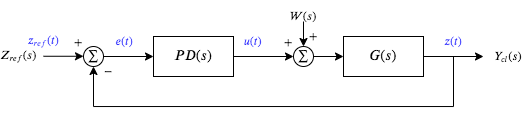
\includegraphics[width=12cm]{img/bdd_1d_noise.png}
\caption{Block diagram of feedback control system with plant noise\label{fig:bdd_1d_noise}}
\end{figure}

Then the equation for the error is similar to \cite[p. 183]{franklin}:

\begin{equation} \label{eq:plantnoise}
E_{cl}(s) = Z_{ref}(s) - Y_{cl}(s) = Z_{ref}(s) - \left( \frac{PD(s) \cdot G(s)}{1 + PD(s) \cdot G(s)} Z_{ref}(s) + \frac{G(s)}{1 + PD(s) \cdot G(s)} W(s) \right)
\end{equation}

There is no tracking error for the given control objectives, so only external disturbances will drive a steady-state error. The last term in eq. \ref{eq:plantnoise} shows the transfer function for noise, and it is clear that increasing the magnitude of $PD(s)$ will decrease the magnitude of the error due to noise. Without a model for the bias/noise, it is hard to say anything about the size of the error. However, if the system is too impacted by noise, $PD(s)$ should be increased. Had noisy sensors been used, increasing $PD(s)$ would however have the adverse effect of amplifying the sensor noise. So there is a design trade-off here.


\section{Closed-loop control}

Putting the physical model and the PD-controller together with closed-loop feedback yields the following system. Here, zero plant noise is assumed.
Recall, the sensors are assumed ideal, so there is unity feedback and also no sensor noise. 

\begin{figure}[H]
\centering
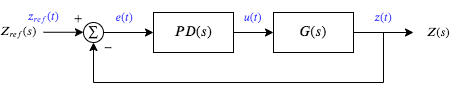
\includegraphics[width=12cm]{img/bdd_1d.png}
\caption{Block diagram of feedback control system\label{fig:bdd_1d}}
\end{figure}

\subsection{Closed-loop transfer function and poles}
The closed-loop system transfer function is given by

\begin{equation} \label{eq:PD_1d_tf}
G_{cl}(s) = \frac{Z(s)}{Z_{ref}(s)} 
= \frac{PD(s) \cdot G(s)}{1 + PD(s) \cdot G(s)}
= \frac{\left(K_d s + K_p \right) \left( \frac{1}{ms^2} \right)}{1+\left(K_d s + K_p \right) \left( \frac{1}{ms^2} \right)}
= \frac{\frac{K_d}{m}s^3 + \frac{K_p}{m} s^2 }{s^4 + \frac{K_d}{m} s^3 + \frac{K_d}{m} s^2}
\end{equation}

Do note that eq. \ref{eq:PD_1d_tf} has fractions in the numerator and demoninator arising from the double integrators. To get a polynomial form, these fractions have been eliminated by multiplying $\frac{s^4}{s^4}$ similar to how \MATLAB~does.
This keeps the structure that the plant has double poles at $s=0$.

Using untuned ``guesstimated'' gain parameters, the system is analyzed with \MATLAB.  \\

\begin{lstlisting}[language=Matlab, style=Matlab-editor]
s = tf('s');    
m = 0.063;          	% mass of drone in kg
G = (1/m)*(1/s^2);  	% G(s), quadrotor-plant
Kp = 0.05;          	% Proportional gain
Kd = 0.1;           	% Derivative gain
PD = Kp + Kd*s;     	% PD(s), PD-controller
Gcl = PD*G/(1+PD*G)   	% G_cl(s), closed-loop system
step(Gcl)
\end{lstlisting}

The closed-loop system with the chosen values for $K_p$ and $K_d$ yields the numeric transfer function.

\begin{equation} \label{eq:PD_1d_tf_num}
G_{cl}(s) = \frac{1.587 s^3 + 0.7937 s^2}{s^4 + 1.587 s^3 + 0.7937 s^2} 
= \frac{s^2 \left(1.587 s + 0.7937 \right)}{s^2 \left(s^2 + 1.587 s + 0.7937 \right)}
\end{equation}

For this choice of $K_p$ and $K_d$, the system poles and zeros are 

\begin{align*}
p_i &= \left\lbrace 0, 0, -0.7937 + 0.4047j, -0.7937 - 0.4047j \right\rbrace \\
z_i &= \left\lbrace 0,0,-0.5 \right\rbrace
\end{align*}

The double poles at the origin are cancelled by the double zeros. 
The two other \gls{LHP} poles could also be found using $p_i = -\frac{K_d}{2m} \pm \frac{\sqrt{K_d^2 - 4 m K_p}}{2m}$ as discussed in the stability section. 
The zero could be found using $z=-\frac{K_p}{K_d}$.

The system is stable as poles are in the \gls{LHP}.
There are no \gls{RHP} zeros, so the system is minimum-phase for any choice of $K_p, K_d > 0$.


\subsection{Closed-loop step response}
The step response for $G_{cl}(s)$ below illustrates how the quadrotor settles at hover at the desired vertical position $z_\text{ref}=1$ \si{\meter}. There is no steady-state error, and no need for adding integral gain, as discussed earlier.


\begin{figure}[H]
\centering
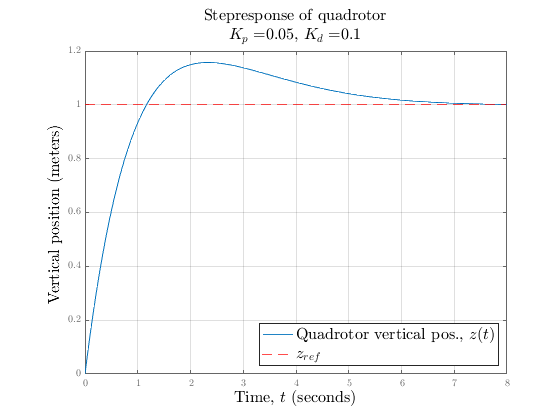
\includegraphics[width=12cm]{img/step_1d.png}
\caption{Step response of quadrotor\label{fig:step_1d}}
\end{figure}

The response has rise time $t_r = 0.86$ sec., but a slow settling time $t_s = 5.9$ sec. and overshoot of 16\%. 
So the PD-controller needs tuning to perform better, especially waiting 6 sec. for the drone to settle at target height is too slow.




\subsection{Test of closed-loop system}
The quadrotor can be driven by any reasonable input, and achieve zero steady-state error when driven by polynomials of up to 1st order (or inputs approximated as such). To test the limits, a sine with an offset is used to drive the system (it is kind of 2nd order in nature, at least piecewise): \\

\begin{lstlisting}[language=Matlab, style=Matlab-editor]
t = 0:1/100:20;         % time vector
z_ref = 1+0.2*sin(2*t);	% oscillate around 1 m with 0.2 m amplitude
z_ref(end-200:end) = 0; % time offset
z_ref(1:200) = 0;       % landing
lsim(Gcl, z_ref, t);	% linear simulation
\end{lstlisting}

\begin{figure}[H]
\centering
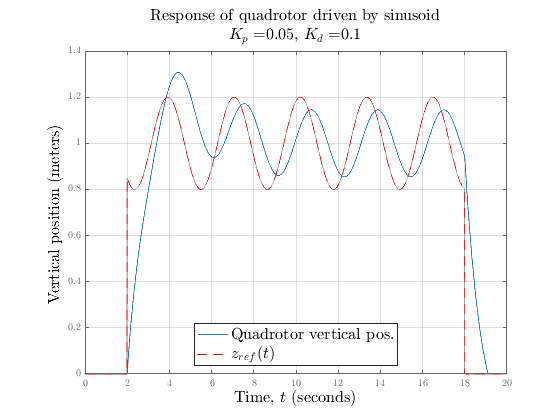
\includegraphics[width=12cm]{img/sin_1d.png}
\caption{Sine response of quadrotor\label{fig:sin_1d}}
\end{figure}

The figure shows that the controller tracks the input reasonably well. It is a bit slow, so there is a lag, and the magnitude error will persist.
More concerning: It shows a ``rough'' landing for the quadrotor, and because the model is linear, $z(t)$ unrealistically goes below zero during landing at around $t=19$ sec. 
More tuning is needed!

\section{Implementation in Simulink, thrust-limiting and tuning}

The Simulink implementation of the dynamic model and PD-controller are below. 

\begin{figure}[H]
\centering
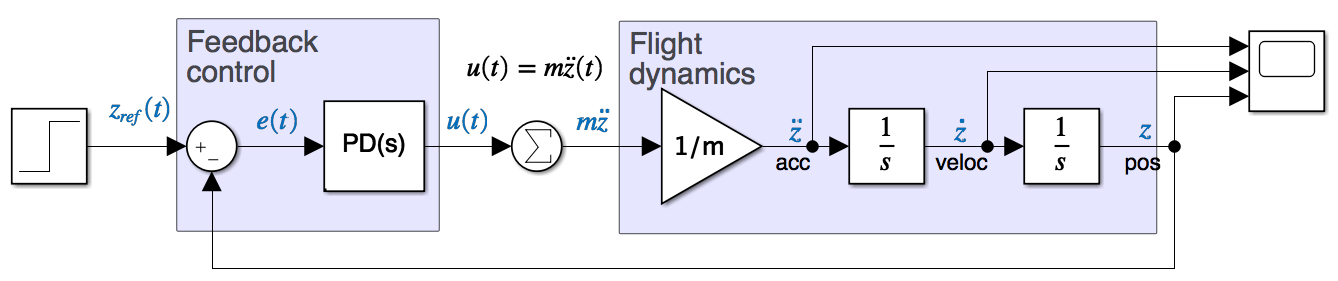
\includegraphics[width=14cm]{img/simulink_1d_1.png}
\caption{Simulink model of 1D dynamics and controller\label{fig:simulink_1d_1}}
\end{figure}

The block diagram is essentially a direct implementation of the \gls{ODE}. This way, it gives insight to internal states of the model.
The first simulation run shown below gives the same step response as seen before.
See the third panel, which shows the position step.
Panels 1 and 2 give a view of internal states (acc is $\ddot{z}$ and veloc $\dot{z}$).

\begin{figure}[H]
\centering
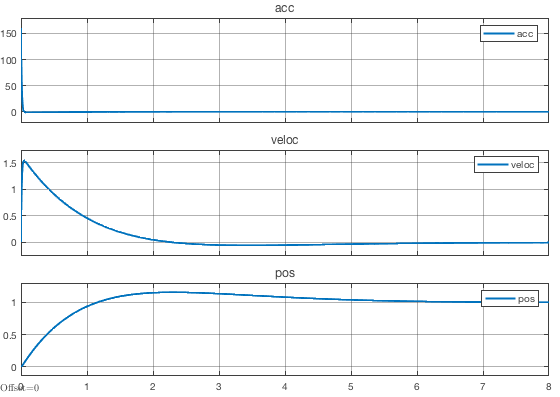
\includegraphics[width=12cm]{img/simulink_1d_sim1.png}
\caption{Simulink linear model simulation (axis 1: time in \si{\second}, axis 2: SI units for the phys. quantity) \label{fig:simulink_1d_sim1}}
\end{figure}

The view of internal states reveals that the acceleration is unrealistically high, initially at about \SI{150}{\newton\per\kilo\gram}. 
At a mass of \SI{63}{\gram} that equates to a force of \SI{9.45}{\newton}.

A more realistic maximum thrust force for this small drone is about \SI{1}{\newton} (assumed), which approximately means that the drone can lift \SI{100}{\gram} including its own weight, i.e. a payload of about \SI{37}{\gram}.

In terms of $u(t)$, the maximum control input is $u_\text{max}(t) = F_\text{max}(t)-mg=1 \text{N} - 0.063 \text{kg}\cdot 9.82 \text{N/kg} = 0.38 \text{N}$. 
That is $\ddot{z}_\text{max}=6$ \si{\newton\per\kilo\gram}.
The minimum control input is $u_\text{min}(t) = F_\text{min}(t)-mg=0 \text{N} - 0.063 \text{kg}\cdot 9.82 \text{N/kg} = - 0.62 \text{N}$.
A limiter is included in the model with these saturation limits, as shown below.

\begin{figure}[H]
\centering
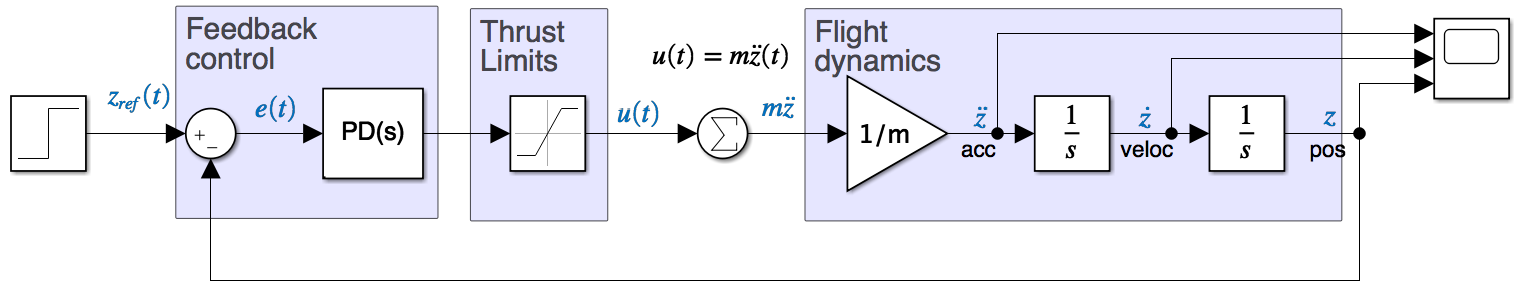
\includegraphics[width=14cm]{img/simulink_1d_2.png}
\caption{Model with nonlinear control input\label{fig:simulink_1d_2}}
\end{figure}

A simulation of this nonlinear model is shown below.

\begin{figure}[H]
\centering
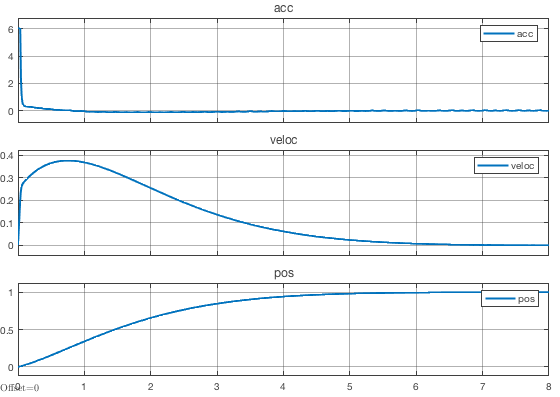
\includegraphics[width=12cm]{img/simulink_1d_sim2.png}
\caption{Simulink nonlinear model simulation (axis 1: time in \si{\second}, axis 2: SI units for the phys. quantity)\label{fig:simulink_1d_sim2}}
\end{figure}

The simulation shows that the acceleration is limited, as wanted.
This nonlinearity has a significant impact on the step response, of course. 
The quadrotor now has a rise time about $t_r = 4$ sec. which is about 4 times longer than the linear model predicted.

\subsection{Tuning}
To tune the controller for better performance, the proportional gain must be \textit{increased} to get a faster system. The derivative gain is then tuned afterwards to manage oscillations.

The Ziegler-Nichols tuning algorithms \cite[p. 206]{franklin} are not used, as the system by itself is not stable: so there is no stable step response to use for the ``quarter decay'' method or ``ultimate gain'' which makes the system marginally stable. So these algorithms won't work. Further, the system being tuned is non-linear.

The tuning is instead done numerically using the Simulink Control Design Toolbox (similar to \texttt{pidtool}). 
A set of tuned PD parameters that give a realistic and acceptable response are $K_p = 0.81$ and $K_d = 0.49$.

The transfer function of the tuned non-linear system is (this time in reduced form):

\begin{equation} \label{eq:PD_1d_tf_num_tuned}
G_{cl, \text{tuned}}(s) = \frac{7.778 s + 12.86}{s^2 + 7.778 s + 12.86} \frac{s^2}{s^2}
\end{equation}

Assuming a linear system, poles and zeros are

\begin{align*}
p_i &= \left\lbrace 0, 0, -5.3943, -2.3835 \right\rbrace \\
z_i &= \left\lbrace 0,0,-1.65 \right\rbrace
\end{align*}

So, disregarding the limiter, the system will be stable (only \gls{LHP} poles).

\section{Test of tuned system with limiter}
The performance of the \textbf{non-linear model} after tuning is shown in the simulation below.

\begin{figure}[H]
\centering
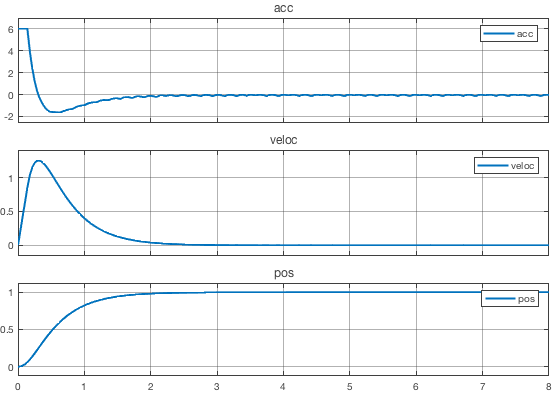
\includegraphics[width=12cm]{img/simulink_1d_sim3.png}
\caption{Tuned controller, nonlinear control input (axis 1: time in \si{\second}, axis 2: SI units for the phys. quantity)\label{fig:simulink_1d_sim3}}
\end{figure}

The figure (third panel) shows the step response. 
Due to the limiter, the response looks like an overdamped or critically damped system, without any oscillations. This matches the poles having zero imaginary part.
Without the limiter, there is an overshoot of about 12 \% (not shown).

The rise time is again back around $t_r = 1$ sec.,
and settling time is a bit below 2 sec., which is realistic for this type of drone. 
The first panel shows how the acceleration $\ddot{z}$ is maxed out during the first part of the step response.

\subsection{Sine response of tuned system}
The final test for this controller is the tracking of a sinewave, including take-off and landing. Same setup as earlier. The result is shown below.
The tuned controller tracks the sine wave much better, despite nonlinearities in the model.
The landing is much less ``rough'' as well, avoiding a crash into to the floor.

\begin{figure}[H]
\centering
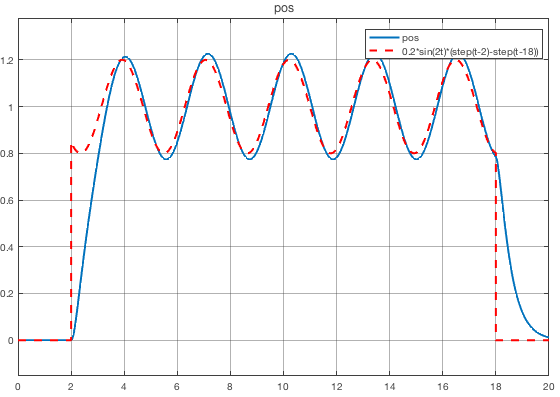
\includegraphics[width=12cm]{img/sin_1d_nonlin_tuned.png}
\caption{Tuned controller, tracking sine wave (axis 1: time in \si{\second}, axis 2: Height in \si{\meter})\label{fig:sin_1d_nonlin_tuned}}
\end{figure}

\newpage
\chapter{Quadrotor in two dimensions}

A second interesting case is to model and control the dynamics of the quadrotor in two dimensions in the $yz$-plane.
Here, the drone can perform roll motion through differential thrust from the rotors, and thereby move from side to side.
The $yz$-plane is the plane seen when looking at the drone head-on. 

\section{Dynamics in the yz-plane}

The idea is to model the flight dynamics and then linearise the equations of motion using a hover configuration and small-angle approximations. 
With that, a linear flight controller can be implemented to manoeuvre the drone to hover at a desired $(y,z)$-position.

\begin{figure}[H]
\centering
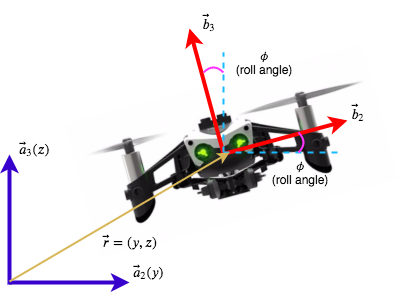
\includegraphics[width=8cm]{img/geo_planar.png}
\caption{Geometry in the $yz$-plane\label{fig:geo_planar}}
\end{figure}

This first figure shows the geometry reduced to the $yz$-plane. 
The drone is constrained to 3 \gls{DoF} as only rotation through the angle $\phi$ is possible. 
It however only has two rotors in the plane, so it is still under-actuated.
In two dimensions, rotation by $\phi$ is as in eq. \ref{eq:rotx} when the 1st axis is removed. 
This gives the rotation matrix, which can transform coordinate vectors in the body frame to coordinate vectors in the world frame.

\begin{equation}
\matr{^\mathcal{A}R_\mathcal{B}} = 
\begin{bmatrix}
\cos\phi & -\sin\phi \\
\sin\phi & \cos\phi
\end{bmatrix}
\end{equation}

The following figure shows the free-body diagram of the planer quadrotor.
On the left figure, thrust is generated by the rotors with magnitude $F_1$ and $F_2$ and same sense as $\vec{b}_3$ in the body frame. Gravity works on the center of mass of the drone with magnitude $mg$ and sense $-\vec{a}_3$ in the world frame.

\begin{figure}[H]
\centering
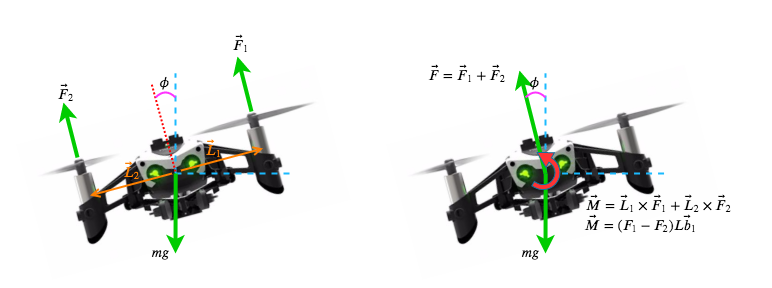
\includegraphics[width=15.5cm]{img/fbd_planar.png}
\caption{Free-body diagram in 2 dimensions\label{fig:fbd_planar}}
\end{figure}

On the right-side figure, the thrusts are decomposed to a pure translational force acting at the center of mass 
and a pure moment (torque on the body) with magnitude $M$ about the center of mass. 

Relative to frame $\mathcal{A}$ (inertial frame), Newton's 2nd law on the center of mass is by eq. \ref{eq:N2}:

\begin{equation}
\sum \vec{F} = 
\begin{bmatrix}
m\ddot{y} \\
m\ddot{z}
\end{bmatrix}_\mathcal{A}
=
\begin{bmatrix}
0 \\
-mg
\end{bmatrix}_\mathcal{A}
+
\matr{^\mathcal{A}R_\mathcal{B}} 
\begin{bmatrix}
  0\\
  F
\end{bmatrix}_\mathcal{B} 
= 
\begin{bmatrix}
  - \sin(\phi) F\\
  -mg + \cos(\phi) F
\end{bmatrix}_\mathcal{A} 
\end{equation}

The pure moment will drive a change in angular momentum of the body, i.e. an angular acceleration $\ddot{\phi}$, around the center of mass. The rotation is about the $\vec{b}_1$-axis of the body frame, where the inertia of the rigid body is $I_{xx}$. The angular acceleration is governed by eq. \ref{eq:rot_kinematics}. Here the vector sense is dropped.

\begin{equation}
\sum \tau = I_{xx} \ddot{\phi} = (F_1-F_2)L = M
\end{equation}

So in all there are three equations of motion for the 3 \gls{DoF}.

\begin{equation}
\begin{bmatrix}
\ddot{y} \\
\ddot{z} \\
\ddot{\phi}
\end{bmatrix}
=
\begin{bmatrix}
  -\frac{1}{m}\sin(\phi) F\\
  -g + \frac{1}{m}\cos(\phi) F \\
  \frac{1}{I_{xx}} M
\end{bmatrix} 
=
\begin{bmatrix}
 0\\
 -g \\
 0
\end{bmatrix} +
\begin{bmatrix}
  -\frac{1}{m}\sin(\phi) & 0\\
  \frac{1}{m}\cos(\phi) & 0 \\
  0 & \frac{1}{I_{xx}}
\end{bmatrix} 
\begin{bmatrix}
 F \\
 M
\end{bmatrix} 
\end{equation}

Similar to the 1-dimensional case, the addition of $\left[ 0, -g, 0 \right]^T$ should be eliminated by variable substitution.
That is, in order to get a linear transfer function for linear inputs $\left[ F, M \right]^T$, the constant term must be eliminated\footnote{
Alternatively, we could also stay with the state-space representation in the time domain.}.
This is a coupled system, because $\phi$ enters in the equations for $y$ and $z$.
As $\phi$ enters non-linearly, the system is non-linear in state due to $\sin\phi$ and $\cos\phi$.
This can be amended with ``small-angle'' approximations.

\subsection{Choosing control inputs}
Control of the drone in 2 dimensions is by way of differential thrusts.
The analysis shows that the total thrust applied will affect the drone in the $\vec{b}_3$ direction in the rotated body frame.
A differential thrust will apply a torque to the body, and thus \textit{rotate} the body frame. 

Two obvious control inputs are available for flight dynamics. One is the sum of thrusts $u_1 = F$ and the other is the moment $u_2 = M$ to roll the drone. The control vector is

\begin{equation} \label{eq:control_vec_nonlin}
 \vec{u} = 
\begin{bmatrix}
u_1 \\
u_2
\end{bmatrix} 
= 
\begin{bmatrix}
F \\
M
\end{bmatrix} 
= 
\begin{bmatrix}
1 & 1 \\
L & -L
\end{bmatrix} 
\begin{bmatrix}
F_1 \\
F_2
\end{bmatrix} 
=
\begin{bmatrix}
F_1 + F_2 \\
(F_1 - F_2)L
\end{bmatrix} 
\end{equation}


The relation between the equations of motion and the control inputs are specified by the combined equations of motion for the 3 \gls{DoF} 

$$
\begin{bmatrix}
\ddot{y} \\
\ddot{z}\\
\ddot{\phi}
\end{bmatrix}
= 
\begin{bmatrix}
0 \\
-g\\
0
\end{bmatrix}
+
\begin{bmatrix}
-\frac{1}{m} \sin\phi & 0 \\
\frac{1}{m} \cos\phi & 0 \\
0 & \frac{1}{I_{xx}}
\end{bmatrix}
\begin{bmatrix}
u_1 \\
u_2
\end{bmatrix} 
$$

\subsection{Linearisation at hover configuration}

The system is linearised around a hover configuration at the origin of $\mathcal{A}$.
Here $(y,z)=(0, 0)$ and $\phi=0$. 
Also, at hover, $u_1(0) = mg$ to exactly counteract gravity.

First, use the small-angle approximation\footnote{For small angles $\cos\phi \approx 1$ and $\sin\phi \approx \phi$.}. 
Second, for horizontal displacement around hover, small changes in \textit{total} thrust can be ignored.
Then, horizontal displacement is driven by the state of $\phi$ alone, and
the first equation becomes $\ddot{y}\approx -\frac{u_1(0)}{m}\phi=-g\phi$. 
The full system is

\begin{equation}  \label{eq:planar_nonlin_sys}
\begin{bmatrix}
\ddot{y} \\
\ddot{z}\\
\ddot{\phi}
\end{bmatrix}
\approx
\begin{bmatrix}
-g\phi \\
-g\\
0
\end{bmatrix}
+
\begin{bmatrix}
0 & 0 \\
\frac{1}{m} & 0 \\
0 & \frac{1}{I_{xx}}
\end{bmatrix}
\begin{bmatrix}
u_1 \\
u_2
\end{bmatrix} 
\end{equation}

To express the system with transfer functions, the constant term $-g$ in the $\ddot{z}$ equation for vertical displacement must be eliminated.
Similar to the 1D case, this is done by the substitution $u_1 = u_1(0) + \tilde{u}_1$, i.e. in terms of deviations from the equilibrium control input.

So the model for vertical displacement becomes $\ddot{z} \approx -g+\frac{u_1}{m} = \frac{\tilde{u}_1 }{m} $.
The full linearised system for which transfer functions can be written is then

\begin{equation} \label{eq:planar_lin_sys}
\begin{bmatrix}
\ddot{y} \\
\ddot{z}\\
\ddot{\phi}
\end{bmatrix}
\approx
\begin{bmatrix}
-g\phi \\
0\\
0
\end{bmatrix}
+
\begin{bmatrix}
0 & 0 \\
\frac{1}{m} & 0 \\
0 & \frac{1}{I_{xx}}
\end{bmatrix}
\begin{bmatrix}
\tilde{u}_1 \\
u_2
\end{bmatrix}
\end{equation}

This begins to look quite similar to a typical state-space representation.
But of course, three more states $\dot{y}$, $\dot{z}$, and $\dot{\phi}$ would be needed to complete the typical first-order form $\dot{\vec{x}} = \matr{A}\vec{x}+\matr{B}\vec{u}$, with $\vec{x}$ being the state-vector, not the $x$-direction.
It is not necessary to complete the state-space here, and is left for future work.

If needed, the thrust per rotor is backed-out by inversion of eq. \ref{eq:control_vec_nonlin}. 
If needed, this could be converted to angular velocities using a model like $F_i = k_F \omega_i ^2$ for rotor.

\begin{equation}
\begin{bmatrix}
F_1 \\
F_2
\end{bmatrix} 
= 
\begin{bmatrix}
\frac{1}{2} & \frac{1}{2L} \\
\frac{1}{2} & -\frac{1}{2L}
\end{bmatrix}
\begin{bmatrix}
u_1 \\
u_2
\end{bmatrix}
=
\begin{bmatrix}
\frac{1}{2} & \frac{1}{2L} \\
\frac{1}{2} & -\frac{1}{2L}
\end{bmatrix}
\begin{bmatrix}
mg+\tilde{u}_1 \\
u_2
\end{bmatrix}
\end{equation}


\section{Transfer functions and s-domain models}

The transfer functions of the three linearised equations of motion are by Laplace transform of eq. \ref{eq:planar_lin_sys}. 

\begin{equation}
G_y(s) = \frac{Y(s)}{\Phi(s)} = -g\frac{1}{s^2}
\end{equation}

\begin{equation}
G_z(s) = \frac{Z(s)}{\tilde{U}_1(s)} = \frac{1}{m} \frac{1}{s^2}
\end{equation}

\begin{equation}
G_{\phi}(s) = \frac{\Phi(s)}{U_2(s)} = \frac{1}{I_{xx}} \frac{1}{s^2}
\end{equation}

First, notice that $G_y(s)$, the transfer function for $y$-direction displacement, is only a response to the roll angle. 
The roll angle transfer function, $G_{\phi}(s)$, is only a response to differential thrust.
The vertical displacement transfer, $G_z(s)$, is only a response to total thrust.

This is of course not fully realistic. 
A more realistic model would keep the coupling of equations and develop the state-space solution. It is outside the scope of this project.

Similar to the 1-dimensional case, all three transfer functions are double integrator plants, i.e. with double poles at the origin of the s-plane. 
So they are also not stable in a BIBO sense, and will require PD-controllers\footnote{
The physical intuition like earlier is that a brief, bounded input at time $t=\delta t$ so $\tilde{u}_1(\delta t)=1$ will cause the quadrotor to accelerate upwards briefly and maintain a constant velocity indefinitely.
The vertical location of the quadrotor would develop according to $z(t)=\frac{1}{m} \int_0^t \int \tilde{u}_1(\tau) d\tau^2 = \frac{1}{2m} t^2 $, tending to $\infty$.
Similar, a brief impulse on $u_2(t)$ would impart an angular momentum on the system, and the rotation would continue indefinitely with constant angular velocity.
Damping terms should be added to remove energy from the system. Better yet, derivative gains.
}.

\section{Implementation of flight dynamics in Simulink}

The flight dynamics (linearised equations of motion) from eq. \ref{eq:planar_lin_sys} is implemented in Simulink as below. 
As the 1D case, it is a straight implementation of the \gls{ODE}s.
Again, notice that the double integrators correspond to the double integration needed to solve the equations of motion with zero initial conditions.

\begin{figure}[H]
\centering
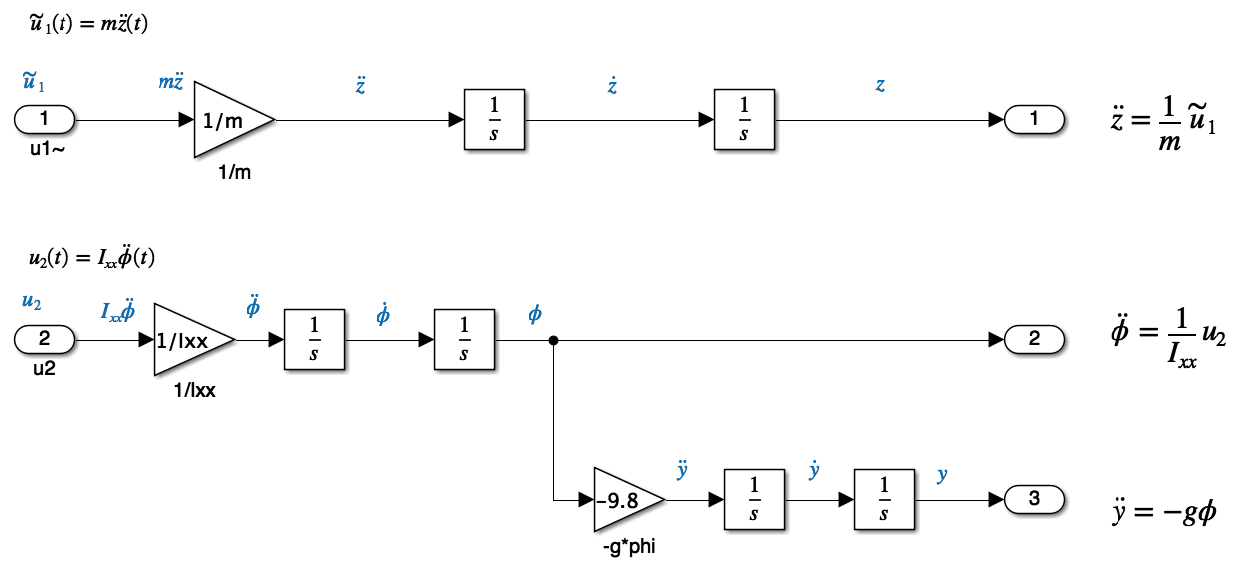
\includegraphics[width=15cm]{img/flight_dyn_2d.png}
\caption{Two-dimensional linearised flight dynamics implemented in Simulink\label{fig:flight_dyn_2d}}
\end{figure}

\section{Controller design}
This time, 3 controllers are needed for the 3 \gls{DoF}.
As in the 1-dimensional case, PD controllers are needed to achieve the hover objectives.
General considerations regarding a PD controller for a double-integrator plant are similar to the earlier case, and not repeated here.

\textbf{Design considerations:} The hover objectives are given as $(y,z)$ coordinates, and $y$ and $z$ controllers need to be the outer controllers. 
These are position controllers.
The state $\phi$ handles the roll of the body to reach the desired $y$-position.
So the roll controller is nested inside the $y$-position controller.

The controller design is shown in the Simulink implementation below. 
The subsystem labelled ``flight dynamics'' contains fig. \ref{fig:flight_dyn_2d}.

\begin{figure}[H]
\centering
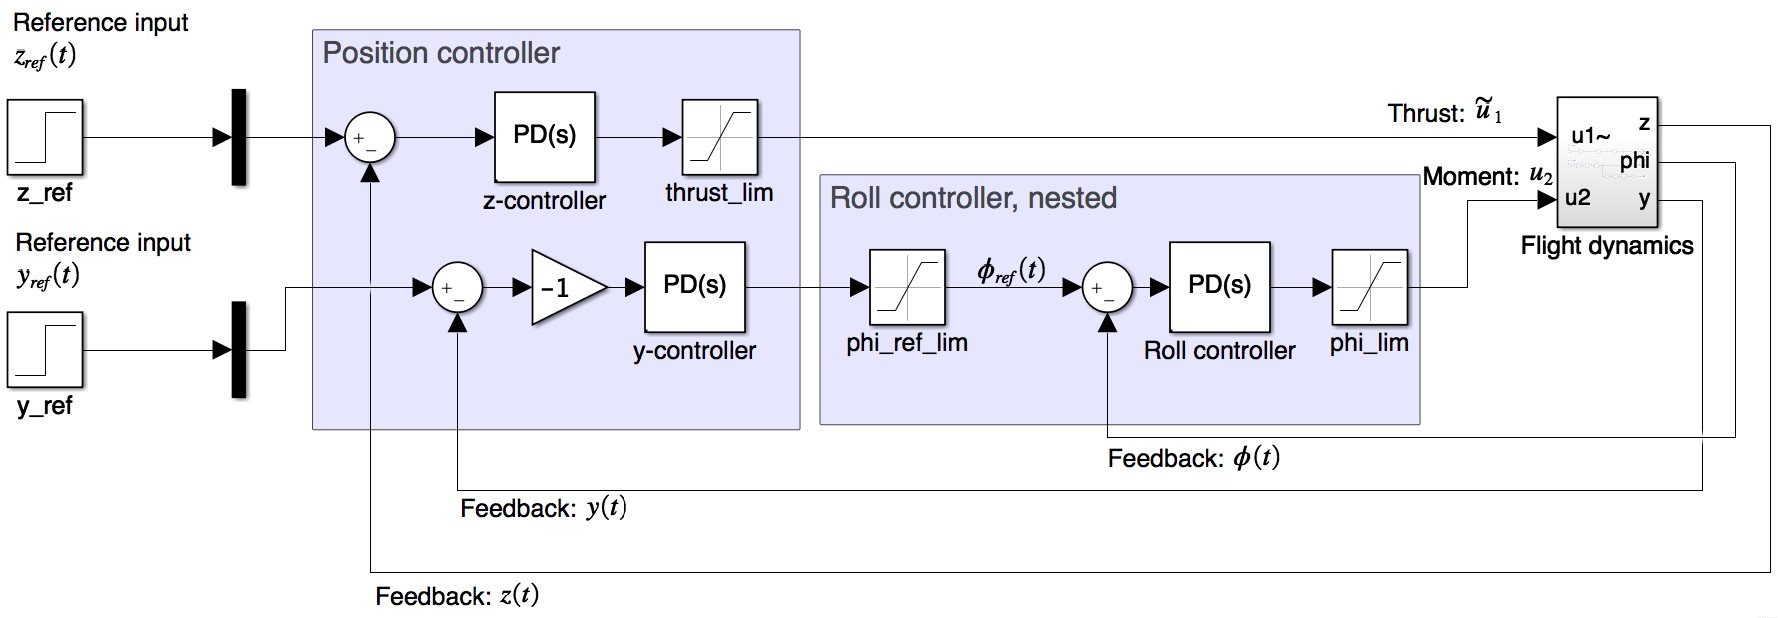
\includegraphics[width=15.5cm]{img/flight_controller_2d.png}
\caption{3-\gls{DoF} controllers for 2D flight dynamics\label{fig:flight_controller_2d}}
\end{figure}

Firstly, the $z$-controller has the same limiter as in the 1D case, as it is essentially the same control problem.

Secondly, notice the inverter before the $y$-controller.
The reason is that for a \textit{positive} $y$-error, $e_y(t)=y_{ref}(t)-y(t)$, the drone position is \textit{to the left} of the desired $y$-position.
The controller therefore must apply a \textit{negative} roll angle in response, in order to move towards the right.

Finally, notice the limiter out of the $y$-position controller, before $\phi_{ref}(t)$ as well as
the limiter out of the roll controller.
They are set at $\pm 0.5$ radians, corresponding to $\pm 30$° to stay within the small-angle approximation\footnote{Here, $\sin(0.5)=0.48$, which is relatively okay.}. 
This way, the position controller will never \textit{set} a large angle, and the roll controller will never \textit{command} a large angle.


\section{Controller tuning}

The values for the $z$-controller are chosen as in the 1D case because this axis is unrelated to the other controllers.

The tuning is done numerically and iteratively using the Simulink Control Design Toolbox.
The $y$ and $\phi$ controllers are tuned with the principle that the inner/nested controller must be faster than the outer controller.
During tuning, the inner controller is tuned towards ``fast'' and ``aggressive'', while 
the outer controller is tuned towards ``slow'' and ``robust''.
The filter order for the Roll controller had to be increased to around 1000 to have a reasonable performance.

Tuned parameter values can be seen in the table.

\begin{table}[h!]
\centering
\begin{tabular}{ |p{5cm}||p{3cm}|p{3cm}|p{3cm}|  }
\hline
\multicolumn{4}{|c|}{PD-controller values for 3-\gls{DoF} controller} \\
\hline
Controller & Saturation limits & $K_p$ & $K_d$ \\
\hline
$z$-position  & $+0.38$, $-0.62$ & \num{0.81}   & \num{0.49} \\
$y$-position  & $\pm 0.5$              & \num{0.5}     & \num{0.4}  \\
$\phi$-roll     &  $\pm 0.5$              & \num{50}      & \num{0.7} \\
\hline
\end{tabular}
\caption{Tuned controller parameters \label{fig:pd_values}}
\end{table}

\section{Performance testing}

The test is to achieve hover at the position $(y,z)=(1,1)$ in meters. 
This is done by first applying a step $z_{ref}=1$ m at $t=1$ to get the drone airborne.
At $t=2$, a step is put on $y_{ref}=1$ m.
The command vector is $\vec{r}_{ref}(t)=[y, z]^T = [1 \cdot h(t-2), 1 \cdot h(t-1)]^T$, with $h(t)$ being the step function. Step responses are shown in the figure below.

\begin{figure}[H]
\centering
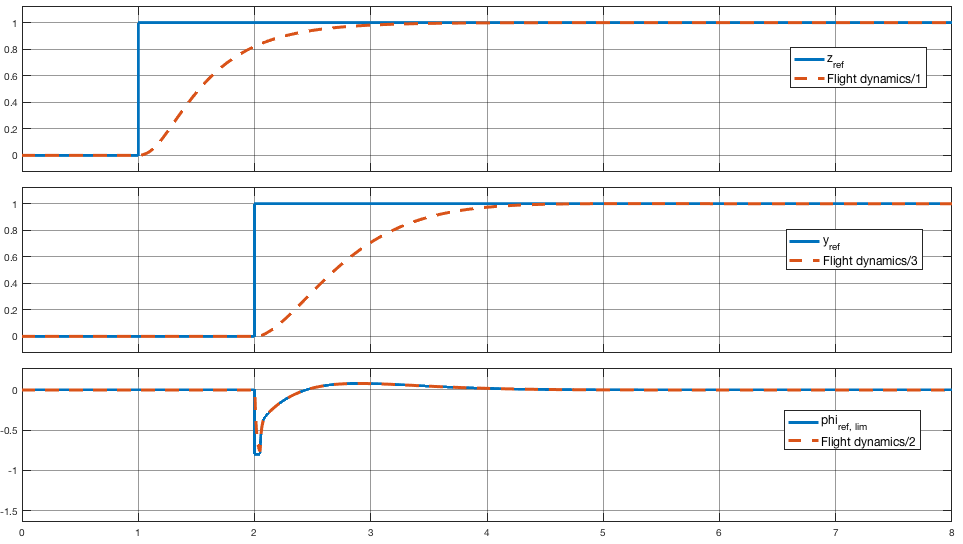
\includegraphics[width=15cm]{img/step_response_2d.png}
\caption{Step responses in the $yz$-plane (axis 1: time in \si{\second}, axis 2: SI units for the phys. quantity)\label{fig:step_response_2d}}
\end{figure}

The trajectory of the drone in the $yz$-plane is in the following figure. 
Axis labels in Simulink's XY-plotter are not easily changed, so here ``X Axis'' corresponds to the horizontal $y$-position, and ``Y Axis'' is the vertical $z$-position.

\begin{figure}[H]
\centering
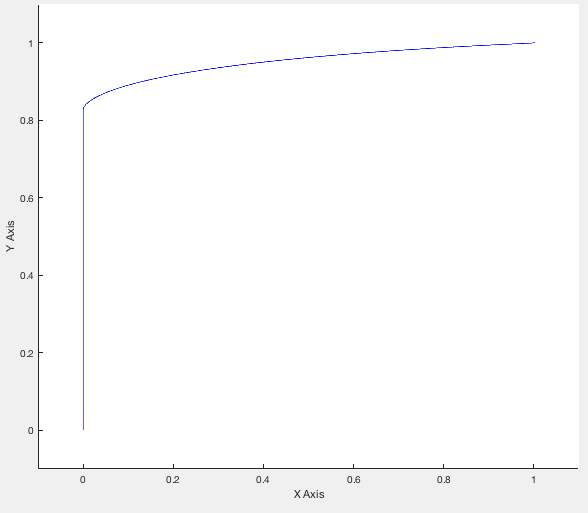
\includegraphics[width=8cm]{img/XY_plot.png}
\caption{Trajectory in the $yz$-plane (axis 1 and 2: Position in \si{\meter})\label{fig:XY_plot}}
\end{figure}

The first figure shows that the step response in the $z$-direction is as before. 
The step response in the $y$-direction is slightly slower, with a rise time at about \SI{1.5}{\second}.
This is believed to be a realistic performance for a small and manoeuvrable drone, probably on the side of too aggressive.
The $\phi$ state shows the expected dynamics: The drone starts out with an aggressive roll with a negative angle, and after about \SI{0.5}{\second} it applies a positive roll to brake and bring its horizontal velocity to zero, until reaching hover at around $t=4$.

All in all, the dynamics and controllers of the system perform as expected in two dimensions.

\newpage
\chapter{Improvements and future work}

The obvious next step is to add full 6 \gls{DoF} dynamics and control. However, due to the extent of the project thus far, the objectives of the project and the complexity in ``doing it right'' with full 3D kinematics, this part was left out. As can be seen from the beginning of the report, it was the intent from the beginning to include 3D.

A simple approach would be to simply add the remaining 3 \gls{DoF} and linearise and decouple exactly as was done in two dimensions. This would require 6 PD-controllers, but wouldn't add anything extra in terms of theoretical value. The best next step would instead be to use a state-space representation in taking the system and application of theory to the next level.

Another clear improvement to the project, which was also cut out due to lack of time, would be to do rigorous testing and improvement of the dynamics and controllers on a real physical quadrotor. The author had in fact acquired a Parrot Mini Mambo for the project. Perhaps there will be time before the exam or in the Summer holiday.

The design of the controller could be changed to a \textit{lead compensation} to get a desired phase margin. 
This would also account for the fact that differentiation in PD is not so physically practical \cite[p. 253]{franklin}.

A key assumption of the methods and models used in this project is that everything is in continuous time. However, the control is done using digital systems, and this should be considered / accounted for by using methods from ``digital control'' \cite[p. 214]{franklin}.

Further consideration regarding disturbances and noise would also make sense. As mentioned in the delimitations, getting usable feedback data from sensors could be an entire project in itself. Also, creating ways to make the drone more robust against disturbances, such as drift from the wind, or handling changes in the terrain, would also be interesting. 

\chapter{Conclusion}

This project has demonstrated how to model the dynamics of a quadrotor in one and two dimensions, and how to linearise the dynamics to get linear systems.
Further, PD-controllers have been designed to achieve stated control objectives.
Even for the relatively simple models in this project, tuning the PD is not a simple matter.

There is still a significant way to go in order to have a fully realistic model, and several improvements and ideas for future work have been identified. It was the aspiration to implement full 3D kinematics and also test on an actual physical quadrotor drone. However, the scope of the project needed to be reduced due to time constraints.

In all, different methods and concepts from control theory have been used to model systems and design controllers. 
In relation to the E4DSE curriculum, system identification from empirical data has of course not been demonstrated as there was no actual physical system.

It was an interesting and useful project. The author intends to continue work on the project when time becomes available.

\cleardoublepage
\chapter{References}
\printbibliography[heading=none]

\newpage

\end{document}

